% OpenAI Math Digest; layout adapted from the repository's Schnell diagrams.
\documentclass[border=12pt]{standalone}
\def\pgfsysdriver{pgfsys-dvisvgm.def}
\usepackage[dvisvgm]{xcolor}
\usepackage{xeCJK}
\setCJKmainfont{HaranoAjiGothic-Regular.otf}[BoldFont=HaranoAjiGothic-Bold.otf]
\setCJKsansfont{HaranoAjiGothic-Regular.otf}[BoldFont=HaranoAjiGothic-Bold.otf]
\usepackage{amsmath,amssymb,tikz,lmodern}
\usetikzlibrary{arrows.meta,positioning,calc}
\renewcommand{\familydefault}{\sfdefault}
\definecolor{ink}{HTML}{25322F}
\definecolor{green}{HTML}{246657}
\definecolor{tint}{HTML}{EEF4F0}
\definecolor{soft}{HTML}{C6D2CC}
\definecolor{muted}{HTML}{52615B}
\newif\ifJapanese
\newcommand{\Tx}[2]{\ifJapanese #1\else #2\fi}
\newcommand{\heading}[2]{{\color{green}\bfseries\Tx{#1}{#2}}\\[5pt]}
\newcommand{\refurl}[2]{\special{dvisvgm:raw <a xlink:href="#1" target="_blank" rel="noopener noreferrer">}{\setlength{\fboxsep}{0pt}\colorbox{white}{\color{green}\underline{\strut #2}}}\special{dvisvgm:raw </a>}}
\newcommand{\OI}[1]{\refurl{https://github.com/openai/math/blob/fd4aeeb2ee4fc729c18d98444fed42fd0529eeeb/preprints/Orbifold-and-logarithmic-Iitaka-subadditivity-September-26-2026/paper.pdf}{#1}}
\newcommand{\Fuj}[1]{\refurl{https://www.math.kyoto-u.ac.jp/~fujino/weak-posi11.pdf}{#1}}
\newcommand{\Cam}[1]{\refurl{https://arxiv.org/pdf/0705.0737v8}{#1}}
\tikzset{
 card/.style={draw=soft,fill=white,rounded corners=2pt,align=left,text=ink,font=\fontsize{10.5}{14}\selectfont,inner xsep=12pt,inner ysep=10pt,text width=14.4cm},
 half/.style={card,text width=6.35cm,minimum height=2.9cm},
 result/.style={card,draw=green,fill=tint,line width=.9pt},
 reason/.style={align=left,text=muted,font=\fontsize{9}{12}\selectfont,inner sep=0pt,text width=12.65cm},
 branchreason/.style={reason,text width=5.65cm},
 edge/.style={-{Stealth[length=2.4mm]},draw=green,line width=1pt},
 wire/.style={draw=green,line width=1pt},
}
% Every vertical arrow has a dedicated left gutter; all labels sit to its right.
\newcommand{\flow}[3]{
 \coordinate (#2-from) at ($(#1.south)+(-6.9,0)$);
 \coordinate (#2-to) at ($(#2.north)+(-6.9,0)$);
 \draw[edge] (#2-from)--(#2-to);
 \node[reason,anchor=west] at ($(#2-from)!.5!(#2-to)+(.55,0)$) {#3};
}

\Japanesefalse
\begin{document}
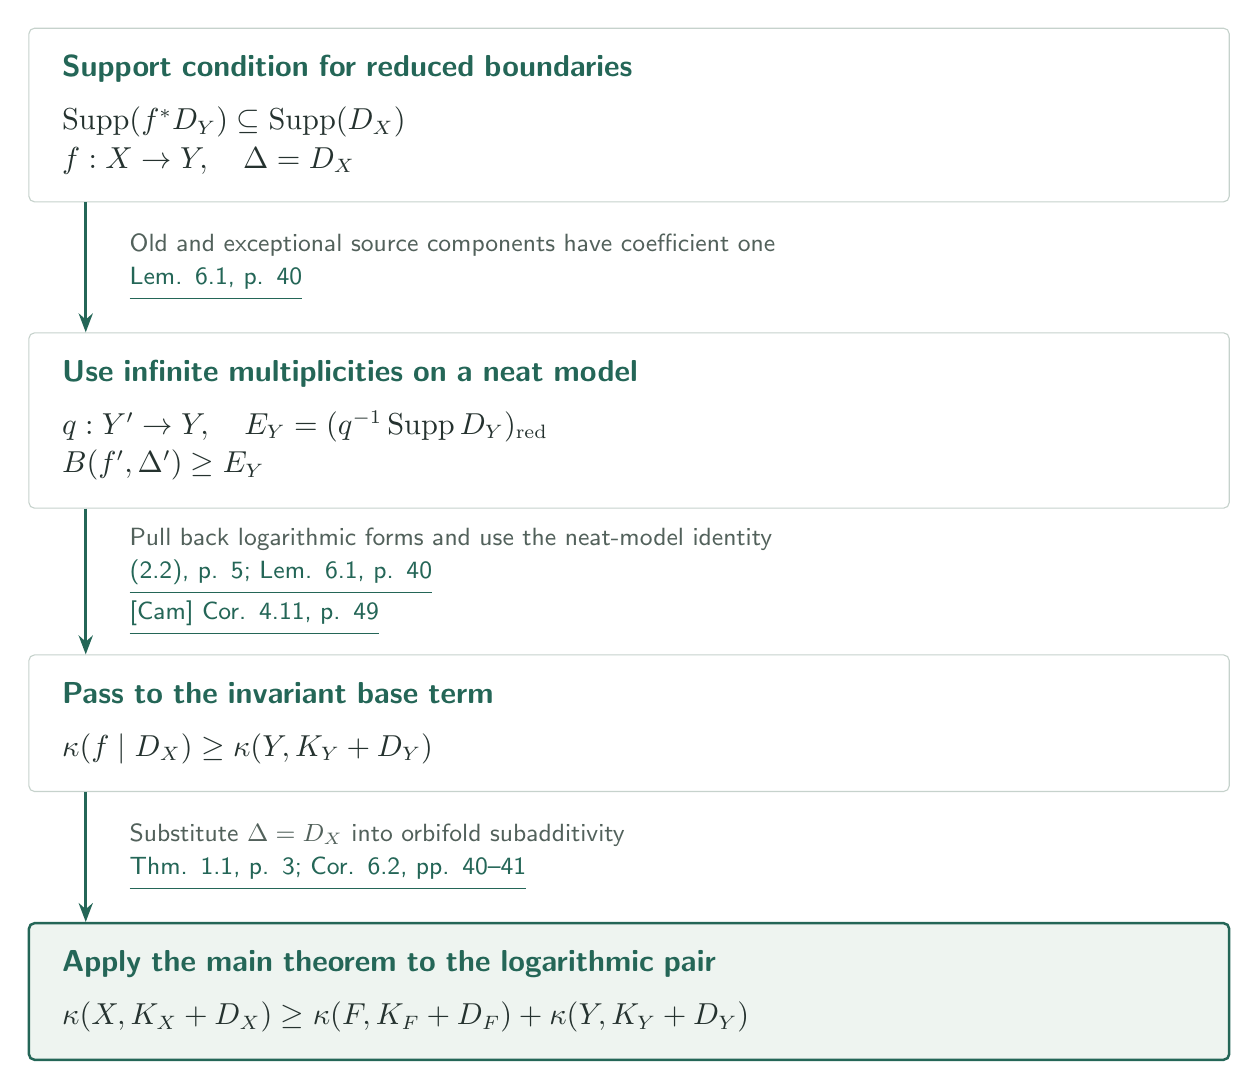
\begin{tikzpicture}
\node[card] (a) {\heading{被約境界の支持条件}{Support condition for reduced boundaries}
 $\operatorname{Supp}(f^*D_Y)\subseteq\operatorname{Supp}(D_X)$\\
 $f:X\to Y,\quad \Delta=D_X$};
\node[card,below=1.65cm of a] (b) {\heading{Neatモデルで無限重複度を使う}{Use infinite multiplicities on a neat model}
 $q:Y'\to Y,\quad E_Y=(q^{-1}\operatorname{Supp}D_Y)_{\mathrm{red}}$\\
 $B(f',\Delta')\ge E_Y$};
\flow{a}{b}{\Tx{旧成分と例外成分に係数1を付けて比較する}{Old and exceptional source components have coefficient one}\\\OI{Lem. 6.1, p. 40}}
\node[card,below=1.85cm of b] (c) {\heading{不変な底項へ移す}{Pass to the invariant base term}
 $\kappa(f\mid D_X)\ge\kappa(Y,K_Y+D_Y)$};
\flow{b}{c}{\Tx{対数形式を引き戻し、neatモデル上の等式を使う}{Pull back logarithmic forms and use the neat-model identity}\\\OI{(2.2), p. 5; Lem. 6.1, p. 40}\\\Cam{[Cam] Cor. 4.11, p. 49}}
\node[result,below=1.65cm of c] (d) {\heading{主定理を対数対に適用する}{Apply the main theorem to the logarithmic pair}
 $\kappa(X,K_X+D_X)\ge\kappa(F,K_F+D_F)+\kappa(Y,K_Y+D_Y)$};
\flow{c}{d}{\Tx{$\Delta=D_X$としてorbifold劣加法性へ代入}{Substitute $\Delta=D_X$ into orbifold subadditivity}\\\OI{Thm. 1.1, p. 3; Cor. 6.2, pp. 40--41}}
\end{tikzpicture}

\end{document}
